\documentclass{article}
\usepackage[utf8]{inputenc}
\usepackage{enumitem}
\usepackage{listings}
\usepackage[margin=0.5in]{geometry}
\usepackage{graphicx}
\usepackage{float}
\graphicspath{ {Images/} }


\title{Physics 111B: \\Error Analysis Lab}
\author{Joshua Levy\\UC Berkeley}
\date{Spring 2017}

\begin{document}

\maketitle

\section{Problems}
    %1
    \subsection{}
    \begin{enumerate}
        \item We want to measure a specific activity with a precision of 1$\%$. This precision corresponds to a fractional error of 0.01. We know the formula for fractional error for a given number N of decays measured is:
            \begin{equation}
                f_e = \frac{1}{\sqrt{N}} = 0.01
            \end{equation}
        Rearranging, and we see that the number of decays that we should find to produce 0.01 fractional error is N = $\frac{1}{0.01}^{2}$ = 10000. We also know the rate at which decays occur can be estimated to be:
            \begin{equation}
                \frac{\Delta N}{\Delta t} = \frac{1000 decays}{5 minutes} 
            \end{equation}
        we will denote the above equation as the constant r, the number of decays rate.\\ The total time it takes to obtain N = 10000 decays, or in order to obtain a fractional error of 0.01, is:
            \begin{equation}
                T = \frac{N}{r} = \frac{10000 decays}{\frac{1000 decays}{5 minutes}} = 50 minutes
            \end{equation}
        So we see that we should measure for 50 minutes in order to obtain a specific activity with a precision of 1$\%$.
    \end{enumerate}
    %2
    \subsection{}
    The following are propagated uncertainties ($\sigma_{Q}$) for Q = \\a) A + B, b) A - B, c) 2A + 2B, and d) A*B, where A and B are distance measurements A $\pm  \sigma_{A}$ and B $\pm  \sigma_{B}$ respectively:
        \begin{enumerate}[label = \alph*]
            \item $\sigma_{Q} = \sqrt{\sigma_{A}^2 + \sigma_{B}^2}$
            \item $\sigma_{Q} = \sqrt{\sigma_{A}^2 + \sigma_{B}^2}$
            \item $\sigma_{Q} = \sqrt{(2\sigma_{A})^2 + (2\sigma_{B})^2} = 2\sqrt{\sigma_{A}^2 + \sigma_{B}^2}$
            \item $\sigma_{Q} = (A*B)\sqrt{(\frac{\sigma_{A}}{A})^2 + (\frac{\sigma_{B}}{B})^2} = \sqrt{(B\sigma_{A})^2 + (A\sigma_{B})^2}$
        \end{enumerate}
    %3
    \subsection{}
        \begin{enumerate}
            \item Sampling the normal distribution N=5 times, we expect the mean ($\bar{x}$) to be 0, the standard deviation to be $\sigma_{x} = 1$, and the error on the mean to be $\sigma_{\bar{x}} = \frac{\sigma}{\sqrt{N}} = \frac{1}{\sqrt{5}} \approx 0.4472$.\\The following code was used to generate a list of 5 normally distributed 5 numbers:
            \begin{lstlisting}[language=Matlab, caption=Matlab code]
            >> a = randn(5,1)
            mean(a)
            std(a)
            std(a)/sqrt(length(a))
            \end{lstlisting}
            which produced the following results: list x = [1.5326, -0.7697, 0.3714, -0.2256, 1.1174], $\bar{x} = 0.4052$, $\sigma_{x} = 0.9431$, and $\sigma_{\bar{x}} = 0.4218$. Computing absolute errors, we see that the observed mean is off by 0.4052, the standard deviation is off by 0.0569, and the error on the mean is off by 0.0254. We see a larger error for the mean (a bit different from what I expected), but smaller errors for the standard deviation and the error on the mean (closer to what I expected). 
            \item Using the MATLAB code featured in the next part for N = 5, the means, standard deviations and errors on the means for each of the M=1000 experiments of N=5 measurements were each found, and a histogram of the data (with 30 bins) is plotted below.
            \begin{figure}[H]
    \centering
    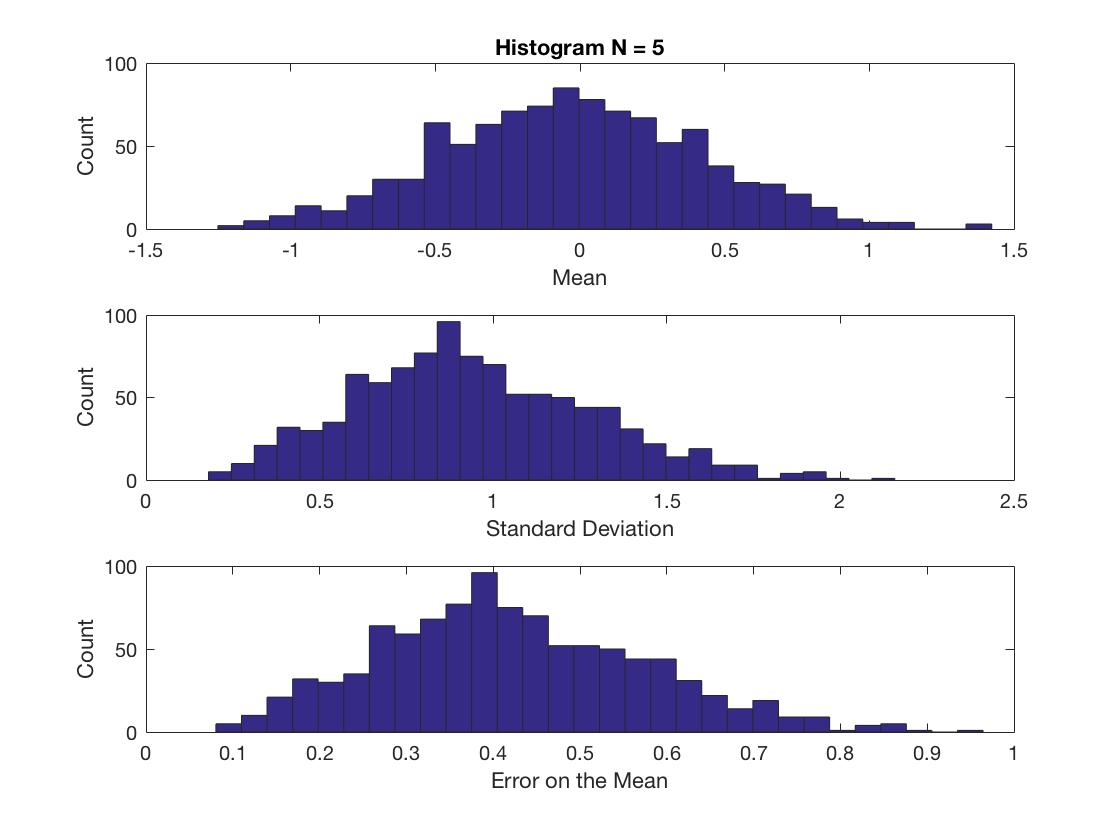
\includegraphics[scale = 0.2]{3a.jpg}
    \caption{Distribution of Means, Standard Deviations, and Errors on the Means for N = 5, M = 1000}
    \label{fig:my_label}
\end{figure}
            Looking at the data tables below the MATLAB code, 67.1\% of the 1000 experiments, or 671 experiments, yielded a result within 1 standard deviation of the true mean of 0. The expected number of experiments to lie within one standard deviation is about 683, so we see that the observed value is close to the expected value. 952 experiments, or 95.2\% of experiments were within 2 standard deviations of the true mean, which is close to the expected value of about 954 experiments. So we see that our observations closely match our expectation.
            \item Parts 1-3 were redone for N=10, 50, 100, 1000. Please see Table 1 for the results. We see that the mean, error on the mean and standard deviations that were observed for one sample fall within expectations, though at lower N values, we see that there are larger deviations between the observed and expected values. 
            \\Generating distributions of means for the other N-values, and we still see that the observed number of experiments falling within one and two standard deviations of the true mean is close to the expected number of experiments. Below are the histograms of those distributions.\\
            \begin{figure}[H]
    \centering
    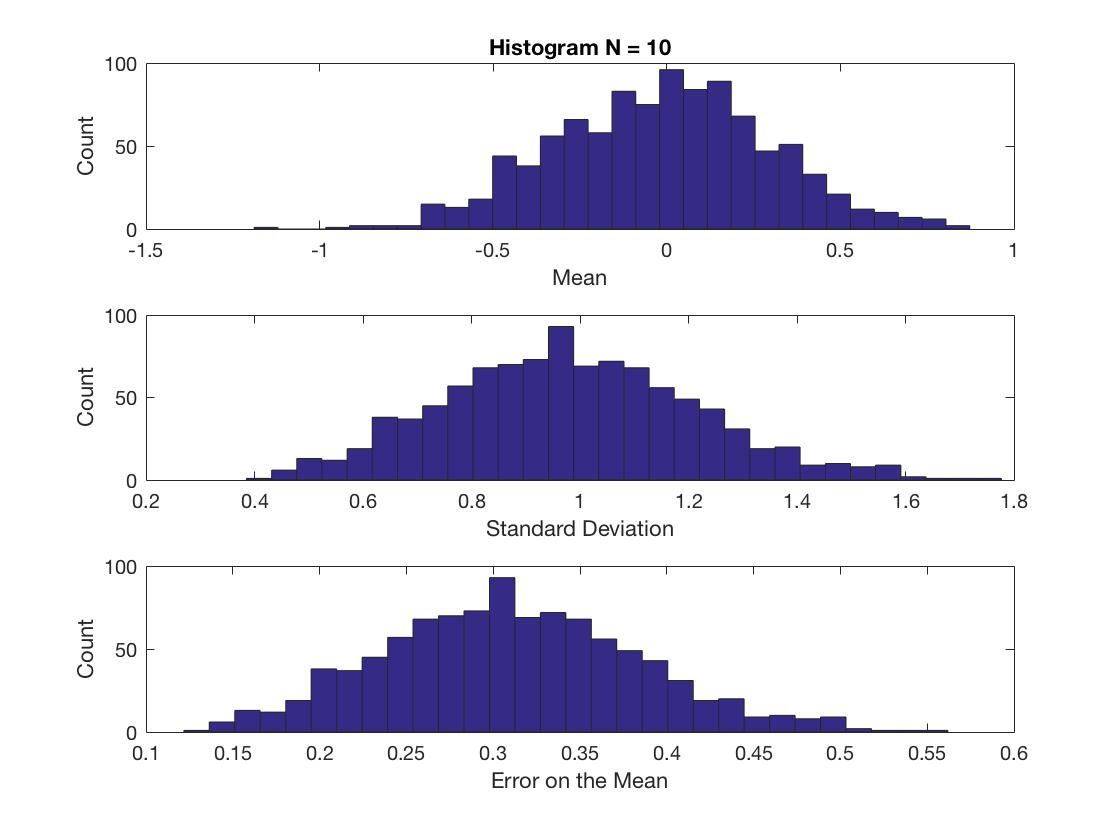
\includegraphics[scale = 0.2]{3b.jpg}
    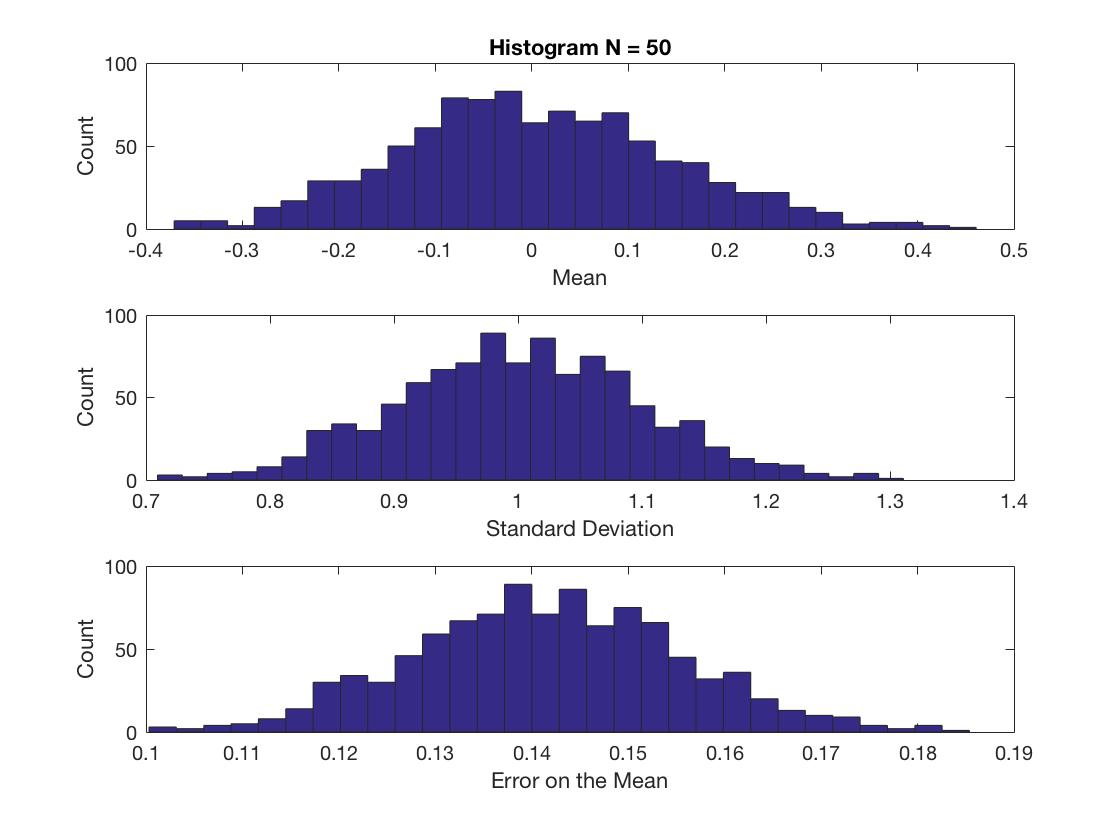
\includegraphics[scale = 0.2]{3c.jpg}
    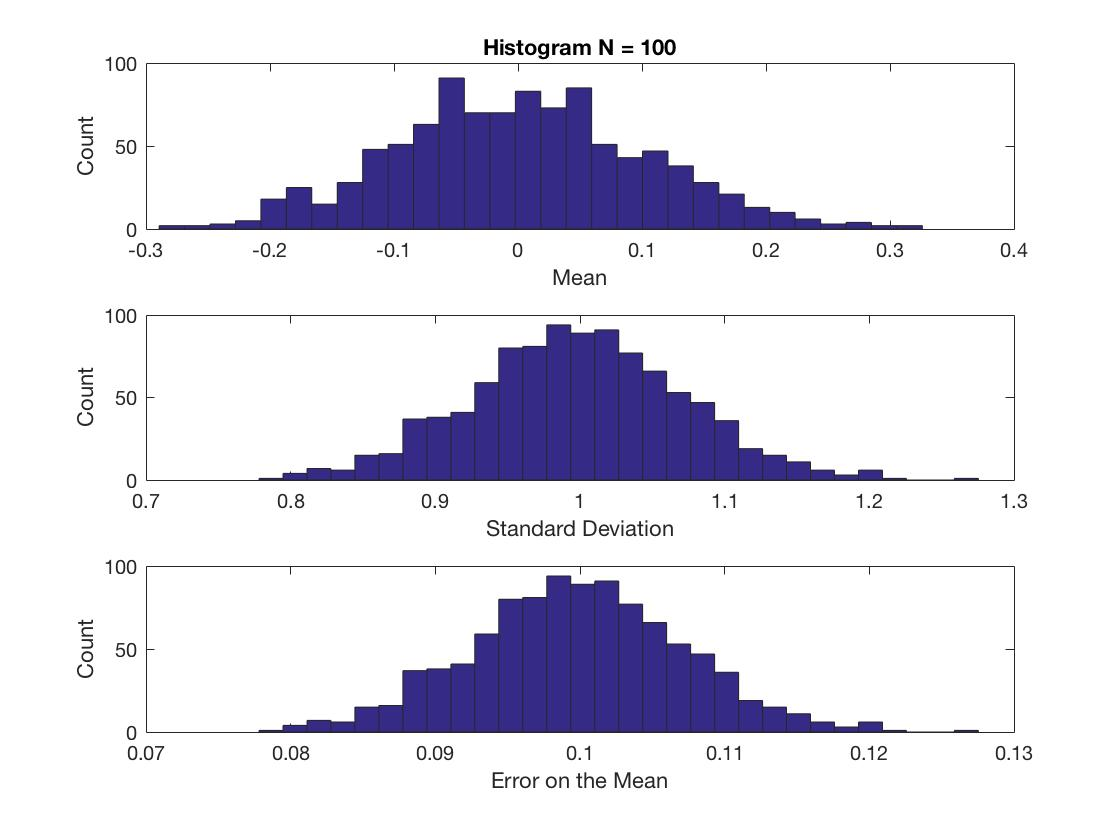
\includegraphics[scale = 0.2]{3d.jpg}
    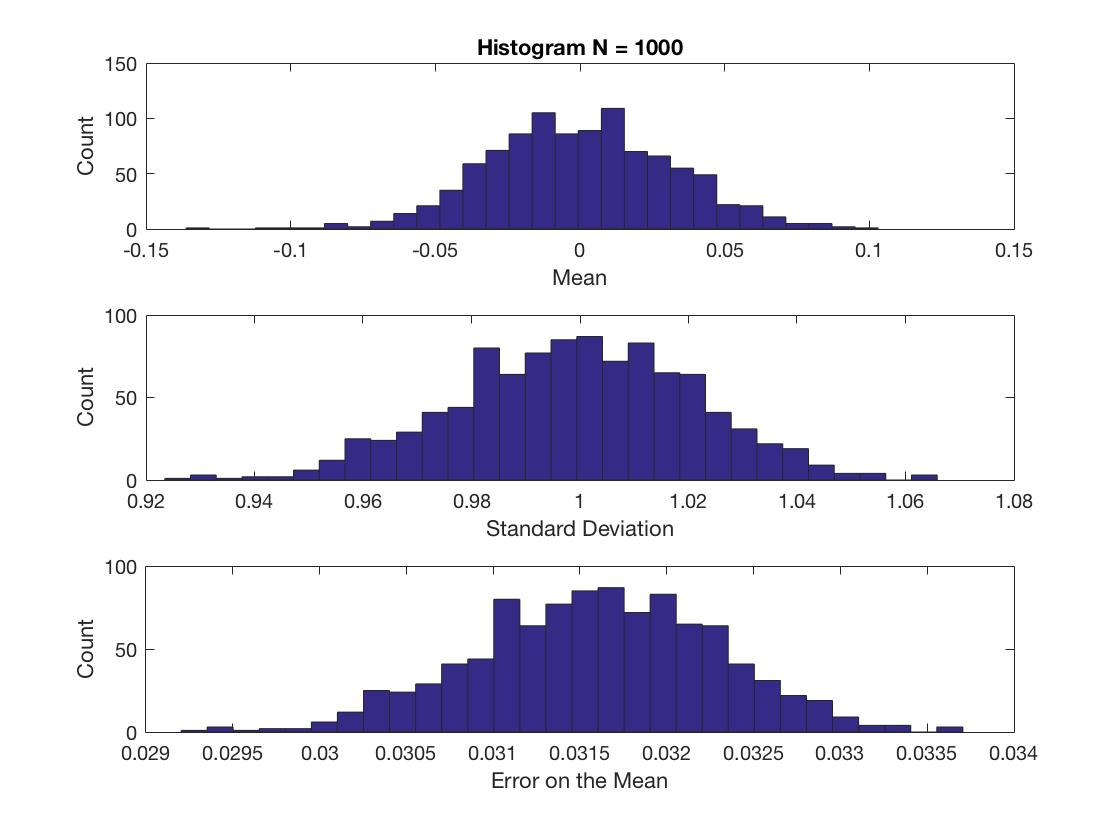
\includegraphics[scale = 0.2]{3e.jpg}
    \caption{Histograms: Distribution of Means, Standard Deviations, and Errors on the Means for N = 10, 50, 100, 1000, and M = 1000}
    \label{fig:my_label}
\end{figure}
            The following code was used to produce the datasets:
            \begin{lstlisting}[language=Matlab, caption=Matlab code]
N = [5,10,50,100,1000];
final = [];
for i=1:length(N)
    a = randn(N(i),1000); m = mean(a); s = std(a); se = std(a)/sqrt(5);
    figure; subplot(3,1,1); hist(m); title(sprintf('Histogram N = %d',N(i)));
    xlabel('Mean'); ylabel('Count'); 
    subplot(3,1,2); hist(s); xlabel('Standard Deviation'); ylabel('Count'); 
    subplot(3,1,3); hist(se); xlabel('Error on the Mean'); ylabel('Count');
    c1 = sum( std(m) > abs(m))/1000 *100;
    c2 = sum( 2*std(m) > abs(m))/1000*100;
    final = [final,[N(i) 0 1 1/sqrt(N(i)) m(1) s(1) se(1) .6826*100. .9544*100. c1 c2]']
end
            \end{lstlisting}
            
            And the table of the other data for the N-values (the last four rows correspond to the M = 1000 lists distributions):
            \begin{table}[H]
            \centering
        \centering
        \caption{Computed Data from Previous Parts}
        \label{my-label}
        \begin{tabular}{llllll}
        \textbf{N} & 5 & 10 & 50 & 100 & 1000 \\
        \textbf{Expected Mean (1 experiment)} & 0 & 0 & 0 & 0 & 0 \\
        \textbf{Expected SD (1 experiment)} & 1 & 1 & 1 & 1 & 1 \\
        \textbf{Expected SE (1 experiment)} & 0.4472 & 0.3162 & 0.1414 & 0.1 & 0.0316 \\
        \textbf{Observed Mean (1 experiment)} & -0.6767 & -0.4912 & 0.0608 & -0.1156 & -0.0184 \\
        \textbf{Observed SD (1 experiment)} & 1.1553 & 1.1257 & 1.0734 & 1.0183 & 1.0066 \\
        \textbf{Observed SE (1 experiment)} & 0.5167 & 0.3560 & 0.1518 & 0.1018 & 0.0318 \\
        \textbf{Expected $\%$ Experiments within 1 SD} & 68.26 & 68.26 & 68.26 & 68.26 & 68.26 \\
        \textbf{Expected $\%$ Experiments within 2 SD} & 95.44 & 95.44 & 95.44 & 95.44 & 95.44 \\
        \textbf{Observed $\%$ Experiments within 1 SD} & 67.1 & 67 & 68.2 & 67.8 & 67.9 \\
        \textbf{Observed $\%$ Experiments within 2 SD} & 95.2 & 95.2 & 95.9 & 95.8 & 95.8
        \end{tabular}
        \end{table}
        \end{enumerate}
    %4
    \subsection{}
        \begin{enumerate}
            \item We begin by utilizing the probability function with the normalized A = 1:
            \begin{equation}
                P(x) = A e^{-x} = e^{-x} 
            \end{equation}
            for x $\geq 0$ and P(x) = 0 for x $<$ 0. The mean, $\bar{x}$ is expected to be:
            \begin{equation}
                \bar{x} = \int_{0}^{\infty} x e^{-x} dx = 1
            \end{equation}
            and the standard deviation is expected to be:
            \begin{equation}
                \sigma_x = \sqrt{\int_{0}^{\infty} (x - \bar{x})^{2} e^{-x} dx} = 1
            \end{equation}
            The standard error on the mean of the distribution (for N = 100) is expected to be:
            \begin{equation}
                \sigma_{\bar{x}} = \frac{\sigma_x}{\sqrt{N}} = \frac{1}{10} = 0.1
            \end{equation}
            Given M=1000 lists of N=100 random numbers, we expect the distribution of means to look like a normal distribution as due the Central Limit Theorem (CLT) because of the large M-value (if M $\geq 30$, CLT can safely be applied). The error of the mean is equal to:
            \begin{equation}
                SE = \frac{\sigma}{\sqrt{N}} = \frac{\sigma}{10}
            \end{equation}
            where $\sigma$ is the standard deviation of the distribution of a sample of N values. If we find the mean of the means (denote as $\mu$) and each individual mean is $\bar{x}_i$ then the standard deviation of the means can be calculated to be:
            \begin{equation}
                \sigma_{\bar{x}} = \sqrt{\frac{1}{M-1}*\sum_i (\bar{x}_i - \mu)^{2}}
            \end{equation}
            However, the standard deviation of means can be estimated by the error on the mean, which was estimated to be 0.1.
            \item Using MATLAB commands a = exprnd(1,100,1), mean(a), and std(a), a list of one hundred exponentially distributed random numbers was generated, with a mean found to be 1.0384 and standard deviation found to be 0.9552.
            \item Using MATLAB commands a = mean(exprnd(1,100,1000)); mean(a), std(a), hist(a); title('Distributions of Means, M = 1000, N = 100, for Random Exponential Distributed Samples'); xlabel('Means'); ylabel('Count');, M=1000 lists of N=100 exponentially distributed random numbers were generated and a histogram of the means was plotted. The distribution appears to look like a normal distribution, which is what was originally thought.  The mean of the distribution was found to be 0.9812 and the standard deviation of the means was found to be 0.0983 of such a distribution. This is close to what we expect because we expect the standard deviation of the means to be close to the error on the mean, which is expected to be 0.1. The histogram for N = 100 is plotted in the next section.
            \item The same calculations in the previous three parts were performed for values of N=1000, 10000. The distribution of means for both looks normal, and a histogram of data for N=100, 1000, 10000 is plotted below:
            \begin{figure}[H]
    \centering
    a)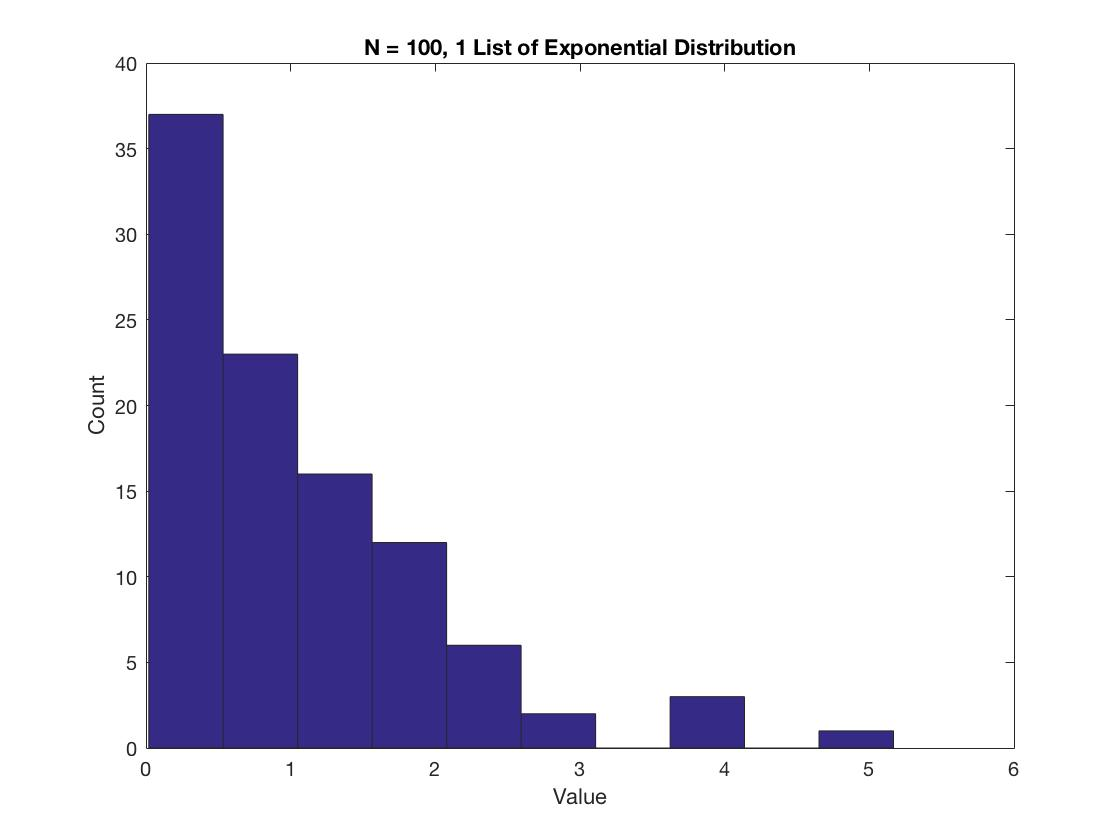
\includegraphics[scale = 0.2]{4a.jpg}
    b)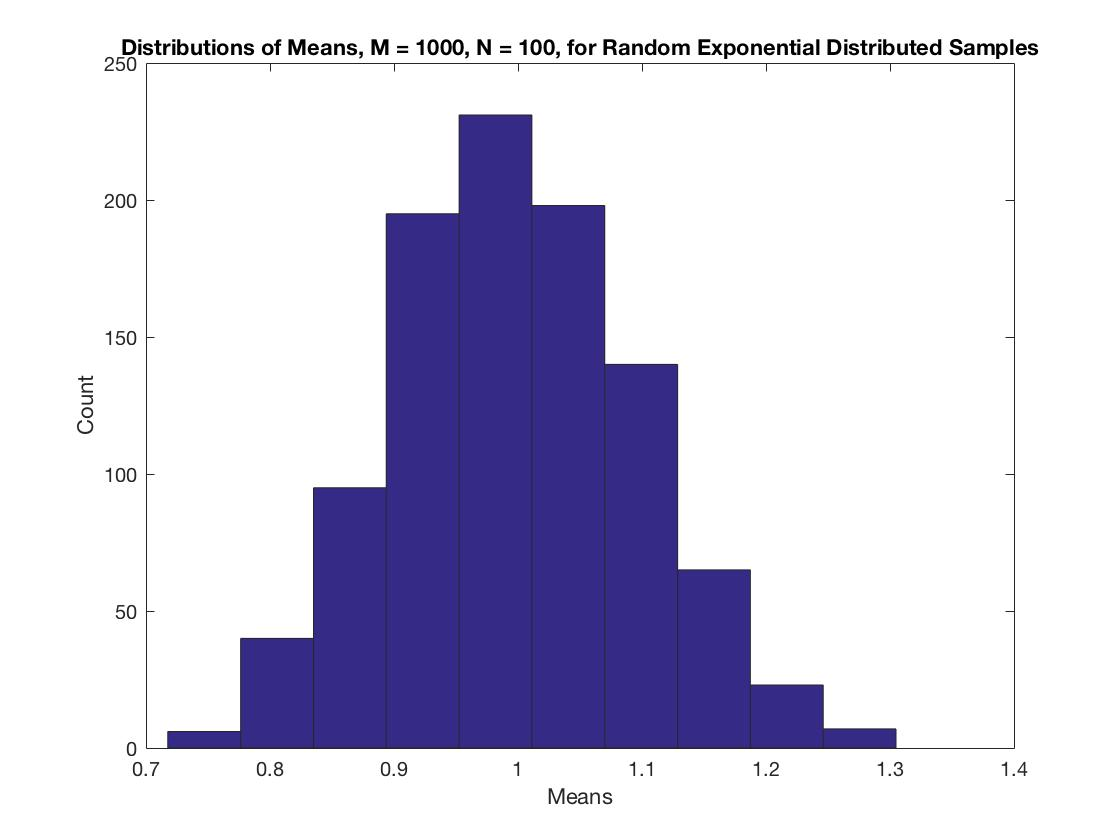
\includegraphics[scale = 0.2]{4b.jpg}
    c)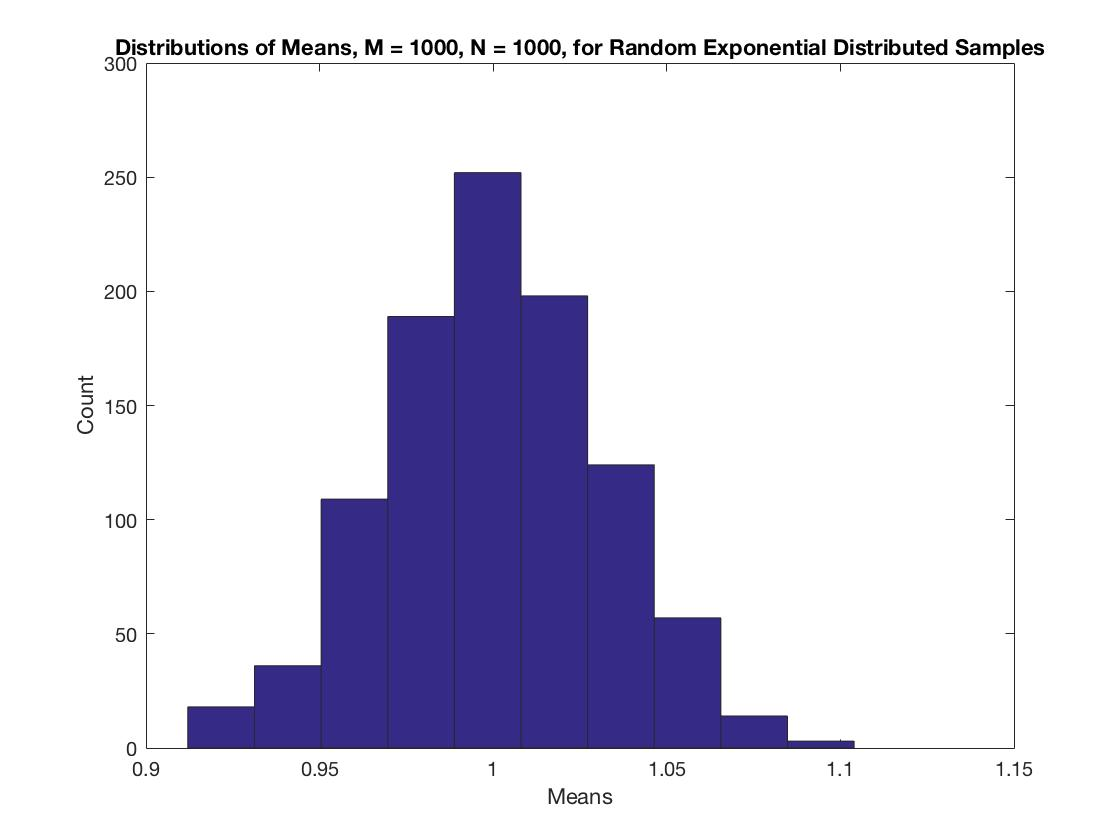
\includegraphics[scale = 0.2]{4c.jpg}
    d)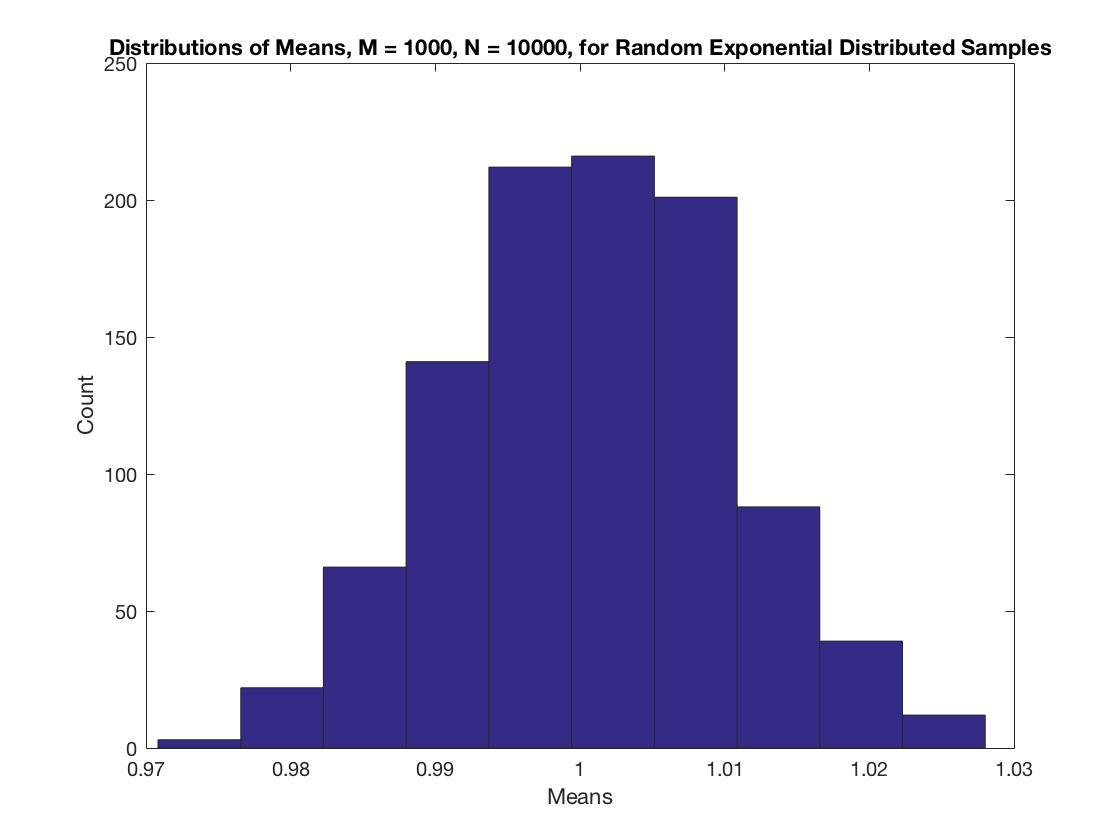
\includegraphics[scale = 0.2]{4d.jpg}
    \caption{a) Histogram of N = 100 Exponential Distribution, One Sample; b-d)Histograms of N = 100, 1000, 10000 and M = 1000 Distribution of Means}
    \label{fig:my_label}
\end{figure}
            The data table that describes the previous three parts for all N values is depicted below:
            \begin{table}[H]
                \centering
                \caption{Data Describing Previous Parts for N = 100, 1000, 10000}
                \label{my-label}
                \begin{tabular}{llll}
                \textbf{N} & 100 & 1000 & 10000 \\
                \textbf{One Experiment- $\bar{x}_{expected}$} & 1 & 1 & 1 \\
                \textbf{One Experiment- $\sigma_{x}expected$} & 1 & 1 & 1 \\
                \textbf{Expected Error On the Mean} & 0.1 & 0.0316 & 0.01 \\
                \textbf{Expected Error On the Mean M = 1000} & 0.1 & 0.0316 & 0.01 \\
                \textbf{One Experiment- $\bar{x}_{observed}$} & 1.0789 & 0.9932 & 0.9959 \\
                \textbf{One Experiment- $\sigma_{x}observed$} & 0.9812 & 0.9516 & 0.9857 \\
                \textbf{Standard Deviation of Means, M = 1000} & 0.0983 & 0.0313 & 0.0095
                \end{tabular}
                \end{table}
                We see that the expected error on the mean for the other N values is close to the observed standard deviation of the distribution of means, so we see that the standard deviation of the distribution of means scales with what we thought by the scaling factor $\frac{1}{\sqrt{N}}$. This demonstrates the Central Limit Theorem.
        \end{enumerate}
    %5
    \subsection{}
    \begin{enumerate}
        \item I produced a histogram with 30 bins that detailed the distribution of energies from the dataset 'peaks.dat'. The data was plotted with error bars for each bin i of error $\sigma_i = \sqrt{N_i}$, where $N_i$ is the total number of entries for a given bin. This was done using the following code:
        \begin{lstlisting}[language=Matlab, caption=Matlab code]
        h1 = histogram(peak,30); hold on;
        errorbar(h1.BinEdges(1:end-1)+mean(diff(h1.BinEdges))/2,h1.BinCounts,sqrt(h1.Values),'o'); hold off;
        \end{lstlisting}
        And produced the following result:
        \begin{figure}[H]
    \centering
    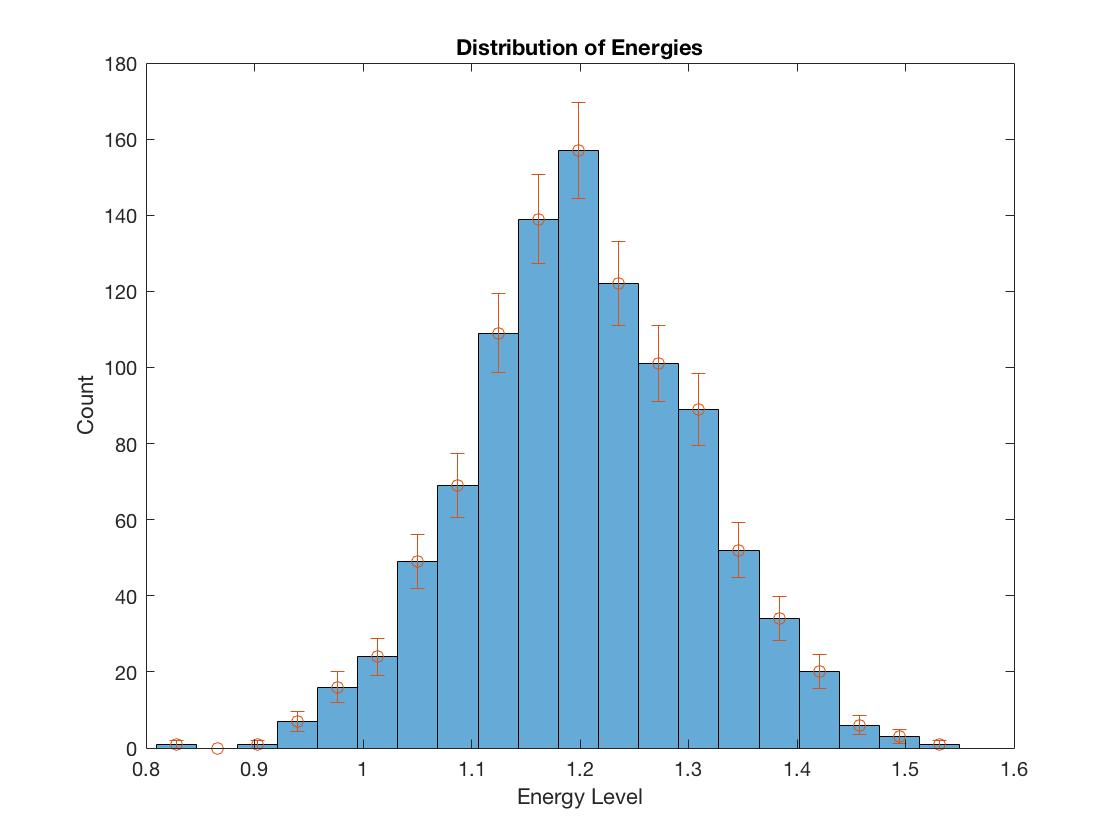
\includegraphics[scale = 0.3]{5a.jpg}
    \caption{Histogram of the Distribution of Energies with n = 30 bins, error bars included}
    \label{fig:my_label}
\end{figure}
        \item The mean and standard deviation of the distribution was found using the MATLAB unbinned gaussian fit command (essentially does statistics on the data): [m,s,mci,sci] = normfit(peak,0.32), yielding a mean of 1.2027 and a standard deviation of 1.038. The 0.32 value used in the code's function corresponds to a 68$\%$ confidence interval (essentially the errors on each metric) for the mean m and standard deviation s. The mean's confidence interval was found to be between 1.1994 and 1.2059, and the standard deviation's confidence interval is between 0.1016 and 0.1062.
        \item We wanted to fit the histogram distribution data to a gaussian curve:
        \begin{equation}
            P(x) = \frac{1}{\sqrt{2*\sigma^2 *\pi}}*e^{\frac{-(x-m)^2}{2*\sigma^2}}
        \end{equation}
        where m and $\sigma$ (can denote as s), the two parameters to be fitted to the x-y data points, correspond to the mean and standard deviation respectively.\\
        We converted the histogram data points into x-y data points, with $x_i$ being the average between the edges of a particular energy level bin, and the count of the energy level bin being $y_i$. The weights of the bins were taken to be the values of the error in each error bar. Then, using MATLAB's curve fitting tool, the data points, along with their weights, were fit to the gaussian function: a*exp(-((x-b)/c)\^{}2), for n = 30 data points. The fit had a correlational $R^2$ value of 0.9164, and "a" was found to be 94.03, "b" was found to be 1.20, and "c" was found to be 0.1441. We see that "b" is the mean (we denote as m), so the fitted mean is fairly close to our calculated mean of 1.2059, falling within the mean's 95\% confidence interval. We see that $c^2 = 2*\sigma^2$, and solving for $\sigma$, we see that the fitted standard deviation $\sigma$ is s = 0.1019, which is within the calculated standard deviation's confidence interval, so the fitted standard deviation agrees with the calculated value.
        \item In the previous exercise, the gaussian function was fit with m and s values. We denote this function as P(x). We want to see how consistent our distribution (histogram data) is with a Gaussian function, so we find the reduced chi-squared value and see how close it is to one. We see that chi-squared is (for n histogram bins):
        \begin{equation}
            \chi^{2} = \sum_{k=1}^{n} \frac{(O_k-E_k)^2}{E_k}
        \end{equation}
        where $E_k$ is the expected value for a given observed bin value/count $O_k$. 
        \begin{equation}
            E_k = N \int_{a_k}^{a_{k+1}} P(x) dx = N*p_k
        \end{equation}
        where N is the total number of measurements or data points, $a_k$ and $a_{k+1}$ are the start and end points of each histogram bin k, respectively, and $p_k$ is equal to the integral expression. On MATLAB, $p_k$ can be coded by using the function integral(@(x) P(x), $a_{k}$, $a_{k+1}$). The reduced chi-squared value is:
        \begin{equation}
            \tilde{\chi}^2 = \frac{\chi^2}{df}
        \end{equation}
        where df is the degrees of freedom, which is the number of measurements minus one.
        Using the code:
        \begin{lstlisting}[language=Matlab, caption=Matlab code]
>> gauss = inline('1/sqrt(2*s^2 * pi)*exp(-1/2*(x-m).^2/s^2)','x','s','m')
chiSQ = 0
for k=1:length(h1.Values)
chiSQ = chiSQ + (h1.Values(k)-1000*integral(@(x) ...
gauss(x,s,m),h1.BinEdges(k),h1.BinEdges(k+1)))^2/(1000*integral(@(x) ...
gauss(x,s,m),h1.BinEdges(k),h1.BinEdges(k+1)));
end
chiSQ_Corrected = chiSQ/29
        \end{lstlisting}
        And we see when we run this code with n = 30, N = 1000, and df = 29 that our reduced chi-squared value equals 1.2998, which is very close to one and indicative of a good fit.
    \end{enumerate}
    
    %6
    \subsection{}
    \begin{enumerate}
    \item The current vs. frequency data is plotted below using MATLAB and a least-squares method (MATLAB polyfit function) was employed to generate the line of best fit, which is also plotted. The equation of this line is:
    \begin{equation}
        f = 3.0540*I + 0.0397 
    \end{equation}
    Here is the plot:
    \begin{figure}[H]
    \centering
    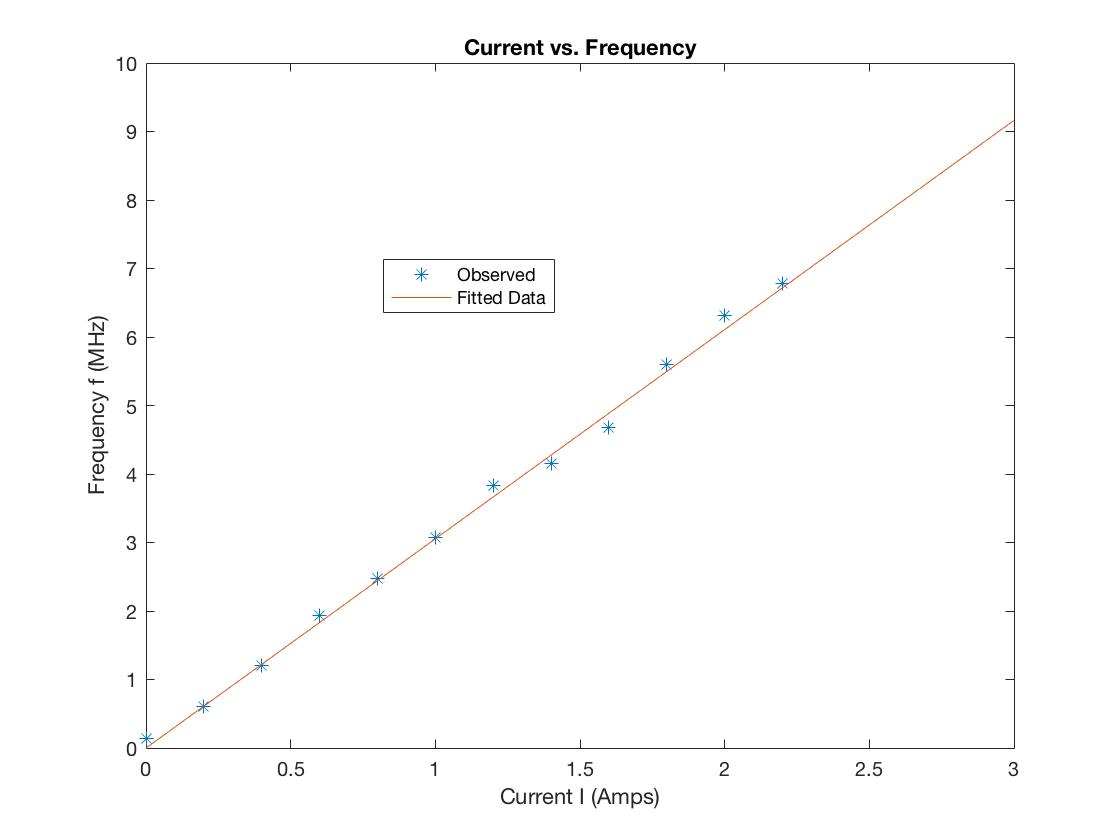
\includegraphics[scale = 0.25]{6a.jpg}
    \caption{Current vs. Frequency Plot, with observed values scattered around fitted line}
    \label{fig:my_label}
\end{figure}
    \item We calculate chi-square of the fit using the following expression:
    \begin{equation}
        \chi^2 = \sum_i \frac{(O_i - E_i)^2}{\sigma_i^2}
    \end{equation}
    where in this case the ith error $\sigma$ is equal to $\sigma_f$=0.01MHz. $O_i$ is an observed frequency data point and $E_i = 3.0540*I_i + 0.0397$. We plug in all of our data points on matlab and find that $\chi^2 = 1.5180*10^3$. Plugging this value and df (degrees of freedom) = 11 into the matlab expression p = 1-chi2cdf($\chi^2$,df), and the probability that the straight line I found is an adequate description of the observed data is estimated to be nearly 0 (bad fit). This is because the error bars we have for each data point is simply too small. If we increase the size of this error to $\sigma_f$=1MHz and run the same computations, $\chi^2$ = 0.1518, and p $\approx$ 1.0, so we see that the data can be described by the model (good fit), because the error is larger and that the line falls within the error bars. 
    \item According to Taylor, the best estimate for the uncertainty in y or frequency f from the scatter of N data points about the best fit line is:
    \begin{equation}
        \sigma_f = \sqrt{\frac{1}{N-2}\sum_{i=1}^N(f_i-(3.0540*I_i + 0.0397))^2}
    \end{equation}
    Plugging in the data points and for N = 12 (number of data points), we calculate this error using the following code on MATLAB: sqrt(sum((o-e).\^{}2)/(10)), where o and e are the observed and expected (using the fitted line) frequency values respectively. This yields $\sigma_f = 0.1232$ MHz. From Taylor, the uncertainty in the slope m ($\sigma_m$) and the intercept b ($\sigma_b$) is calculated using the following expressions:
    \begin{equation}
        \sigma_m = \sigma_y*\sqrt{\frac{N}{\Delta}}
    \end{equation}
    \begin{equation}
        \sigma_b = \sigma_y*\sqrt{\frac{\sum_{i} I_i^2}{\Delta}}
    \end{equation}
    where $I_i$ is the ith current measurement and $\Delta$ is:
    \begin{equation}
        \Delta = N*\sum_{i=1}^N I_i^2 - (\sum_{i=1}^N I_i)^2
    \end{equation}
    Plugging these equations into MATLAB, and we find that $\Delta = 68.6400$, $\sigma_m = 0.0515$ MHz/Amps, and $\sigma_b = 0.0669$ MHz. 
    \item For the weighted best fit line, f = m*I + b, we learn from Taylor that:
    \begin{equation}
        m = \frac{(\sum_{i=1}^N w_i)*(\sum_{i=1}^N w_i*I_i*f_i) - (\sum_{i=1}^N w_i * I_i)*(\sum_{i=1}^N w_i*f_i)}{\Delta}
    \end{equation}
    \begin{equation}
        b = \frac{(\sum_{i=1}^N w_i*I_i^2)*(\sum_{i=1}^N w_i*f_i) - (\sum_{i=1}^N w_i * I_i)*(\sum_{i=1}^N w_i*I_i*f_i)}{\Delta}
    \end{equation}
    where $f_i$ is the ith observed frequency, $I_i$ the ith observed current, and $w_i$ and $\Delta$ are:
    \begin{equation}
        w_i = \frac{1}{\sigma_f^2} = \frac{1}{(0.03 + 0.03 * f_i)^2}
    \end{equation}
    \begin{equation}
        \Delta = (\sum_{i=1}^N w_i)*(\sum_{i=1}^N w_i*I_i^2) - (\sum_{i=1}^N w_i * I_i)^2
    \end{equation}
    and with N=12, we plug in these equations into MATLAB using relevant expressions (with I denoted as x and f denoted as y), 
    \begin{lstlisting}[language=Matlab, caption=Matlab code]
>> w = arrayfun(@(z) 1/(0.03 + z*0.03)^2,y)
delta = sum(w)*sum(w.*x.^2)-(sum(w.*x))^2
m = (sum(w)*sum(w.*x.*y)-sum(w.*x)*sum(w.*y))/delta
b = (sum(w.*x.^2)*sum(w.*y)-sum(w.*x)*sum(w.*x.*y))/delta
    \end{lstlisting}
    and find that $m\approx 2.9905$ MHz/Amps and $b\approx 0.0892$ MHz, which are the slope and intercept of the best-fit line using the least-squares method with unequal weights.
    \end{enumerate}
    %7
    \subsection{}
    \begin{enumerate}
        \item Suppose the muon decay rate as a function of time could be measured using data points $(x_i,y_i)$, where x is time and y is decay rate. This decay rate can be modelled by:
        \begin{equation}
            y = Ae^{-Bx}
        \end{equation}
        and taking the logarithm of both sides and denoting ln(y) = z, we can apply a best-fit line to the data:
        \begin{equation}
            z = ln(y) = -Bx + ln(A) 
        \end{equation}
        The statistical error $\sigma_i$ or $\sigma_y$ ascribed to any $y_i$ data point is transformed as the natural log is taken:
        \begin{equation}
            \sigma_z = |\frac{dy}{dz}|*\sigma_y = \frac{\sigma_y}{y}
        \end{equation}
        So when the semi-log histogram is plotted, we see that the statistical uncertainty decreases as y increases. So if $y_i$ is reasonably large, the uncertainties that we will be getting will decrease towards 0 in our ln(y) plot. The error will start out as large near low y values and decrease as the magnitude of y increases. Qualitatively, transforming the y values will cause the errors on the y measurements to widen or narrow.
        \item In a separate experiment, we find that $\log E_0 = 2.1 \pm .5$. Taking the exponent of both sides, and we see that $E_0 = e^{2.1} \approx 8.166$, and reversing the error propagation equation used above, we see that the error of $E_0$ ($\sigma_{E_0}$), where z = ln($E_0$) and $\sigma_z = 0.5$:
        \begin{equation}
            \sigma_{E_0} = \frac{dE_0}{dz}\sigma_z = e^z*\sigma_z = e^{2.1}*0.5 \approx 4.083
        \end{equation}
        So $E_0$ = 8.166 $\pm$ 4.083.
    \end{enumerate}

\end{document}

Notes: Finish 3 and 4 add figures.. caption CHANGE EQUATIONS AND DERIVATIONS- error on mean problems, ADD UNITS to all problems!!!!
x1,x2,START ADDING FIGURES HERE 3,4,5,6,x7
Monday- finish EAX  
\begin{figure}[H]
    \centering
    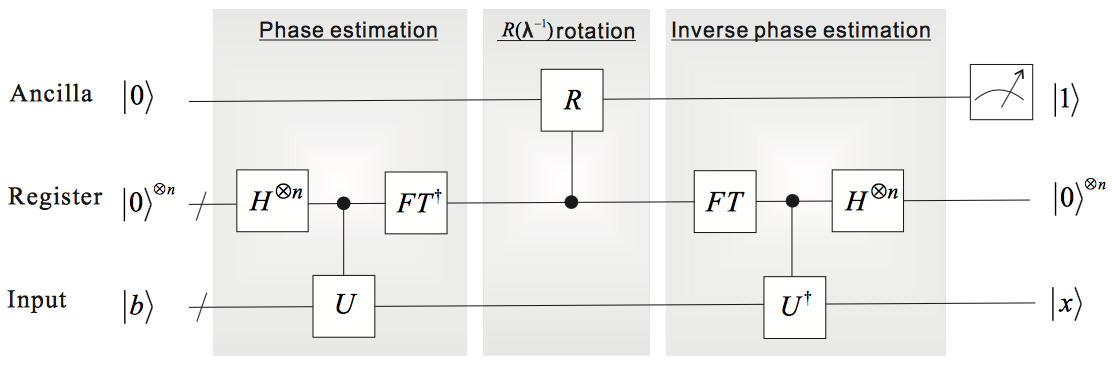
\includegraphics[scale = 0.5]{1.png}
    \caption{Caption \cite{lab11}}
    \label{fig:my_label}
\end{figure}